%%%%%%%%%%%%%%%%%%%%%%%%%%%%%%%%%%%%%%%%%%%%%%%%%%%%%%%%%%%%%%%%%%%%%%%%%%%%%%%
% name:         | neutrality.tex
% @uthor:       | Axel Martin <axel.martin@eisti.fr>
% title:        | Include : Neutralité du net
% brief:        | Explication de la neutralité du net pour la Coding Night
% licence:      | free
% more:         | Warning: inputenc en utf8
%               | Warning: n'oublies pas vos \subsection (3 à 4 maximum)
%%%%%%%%%%%%%%%%%%%%%%%%%%%%%%%%%%%%%%%%%%%%%%%%%%%%%%%%%%%%%%%%%%%%%%%%%%%%%%%


\section{La neutralité du net}
\begin{frame}\frametitle{}
    {\Huge La neutralité du net}

    \vspace{2em}

    Le net c'est bien, mais pourquoi on nous espionne ?
\end{frame}


\subsection{Qu'est-ce que c'est ?}
\begin{frame}\frametitle{Définition}
    \emph{Rappel du principe : chaque noeud d'internet doit être considéré de
        la même manière que les autres, sans distinction de son origine ou du
    groupe qui en est responsable}
    \vspace{1em}

    \begin{itemize}
        \item équité des débits
        \item non appropriation du réseau
        \item respect de la vie privée
    \end{itemize}
\end{frame}


\begin{frame}\frametitle{Une notion bien contestée}
    Comment doit-on réagir face aux sites :
    \begin{itemize}
        \item pédophiles
        \item à incitation terroriste
        \item de vente de drogues (parse ke la drog c male)
    \end{itemize}
\end{frame}


\begin{frame}\frametitle{La réponse}
    \begin{center}
        {\Large C'est pas la censure / la réduction de débit / l'espionnage qui pose problème}

        \vspace{2em}

        {\Large C'est la manière dont c'est fait :)}
    \end{center}
\end{frame}


\begin{frame}\frametitle{Une notion bien ignorée}
    \begin{itemize}
        \item L'espionnage (\textsc{NSA}...)
        \item réduction de débit des FAI (\textsc{YouTube} vs \textsc{Free})
        \item la censure (Chine, Corée du Nord...)
    \end{itemize}
\end{frame}


%%%%%%%%%%%%%%%%%%%%%%%%%%%%%%%%%%%%%%%%%%%%%%%%%%%%%%%%%%%%%%%%%%%%%%%%%%%%%%%
\subsection{De la réduction de débit...}
\begin{frame}\frametitle{L'équité des débits}
    \emph{Rappel du principe : chaque noeud d'internet doit être considéré de
        la même manière que les autres, sans distinction de son origine ou du
    groupe qui en est responsable}
    \begin{itemize}
        \item pas de bridage par rapport à un critère (opérateur, fournisseur...)
    \end{itemize}
\end{frame}


\begin{frame}\frametitle{Le mauvais futur : un internet à deux débits}
    % TODO : inclusion de l'image des route
\end{frame}


\begin{frame}\frametitle{Mais est-ce déjà en application ?}
    \begin{itemize}
        \item \textsc{Google} et \textsc{Free}
        \item \textsc{NetFlix} qui paye plus chez certains fournisseurs pour une meilleure bande passante
    \end{itemize}
\end{frame}


\begin{frame}\frametitle{Pourquoi font-ils cela ?}
    \emph{Raisons évoquées par les opérateurs :}
    \begin{itemize}
        \item limitation de la saturation du réseau
        \item rentabilisation du réseau\\
    \end{itemize}

    \textbf{Question ouverte : } Mais si les opérateurs peuvent fournir un
    accès rapide pour un site, ils peuvent le fournir pour tous les sites non ?
\end{frame}


%%%%%%%%%%%%%%%%%%%%%%%%%%%%%%%%%%%%%%%%%%%%%%%%%%%%%%%%%%%%%%%%%%%%%%%%%%%%%%%
\subsection{... en passant par la censure...}
\begin{frame}\frametitle{Un internet accessible à tous et pour tous}
    \emph{Rappel du principe : chaque noeud d'internet doit être considérér de
        la même manière que les autres, sans distinction de son origine ou du
    groupe qui en est responsable}

    \vspace{1em}

    \begin{itemize}
        \item chaque noeud est autant accessible qu'un autre
        \item pas de distinction par rapport au contenu proposé par le noeud
    \end{itemize}
\end{frame}


\begin{frame}\frametitle{Le cas de la Corée du Nord}
    \begin{itemize}
        \item un internet fermé
        \item fortement censuré
        \item centralisé
    \end{itemize}

    \vspace{1em}

    \color{red}\emph{Contraire à toutes les définitions de la neutralité du net}
\end{frame}


\begin{frame}\frametitle{Le cas de la Chine}
    \begin{itemize}
        \item un internet ouvert au monde...
        \item ...mais avec un bon gros proxy ;)
        \item partiellement contrôlé
        \item avec quelques peines de mort qui trainent (le VPN, c'est pas bien)
    \end{itemize}

    \color{red}\emph{Contraire à toute les définitions de la neutralité du net}
\end{frame}


\begin{frame}\frametitle{Et en France ?}
    \begin{itemize}
        \item la loi \textsc{LOPSI} permet de filter un contenu sans passer
            par une administration juridque
        \item les textes des loi \textsc{SOPA/PIPA} auraient pu permettre ce
            genre de démarches de manière juridique et tout à fait légale
        \item quelques textes <<\emph{secrets}>> pourraient permettre ce genre
            de choses (traité transatlantique)
    \end{itemize}
\end{frame}


%%%%%%%%%%%%%%%%%%%%%%%%%%%%%%%%%%%%%%%%%%%%%%%%%%%%%%%%%%%%%%%%%%%%%%%%%%%%%%%
\subsection{... jusqu'à l'espionage}
\begin{frame}\frametitle{Un internet accessible à tous et pour tous}
    \emph{Rappel du principe : chaque noeud d'internet doit être considéré de
        la même manière que les autres, sans distinction de son origine ou du
    groupe qui en est responsable}

    \vspace{1em}

    \begin{itemize}
        \item les informations transitant d'un noeud à un autre sont privées
        \item les interceptions faites sur ces informations doivent passer par
            une structure judiciaire
    \end{itemize}
\end{frame}


\begin{frame}\frametitle{Interception administrative et interception judiciaire}
    \emph{Qu'est-ce qu'une interception ?}

    $\Rightarrow$ Récupération de donnée transitant sur le réseau ne nous étant
    pas adressé.

    \vspace{1em}

    \textbf{Interception judiciaire :} validation judiciaire requise
    \begin{itemize}
        \item permet de cadrer les interceptions
        \item laisse des traces
        \item lent
    \end{itemize}

    \textbf{Interception administrative :} validation judiciaire non requise
    \begin{itemize}
        \item on ne sait pas ce qui est vraiment intercepté
        \item plein pouvoirs possibles
        \item certes, c'est plus rapide
    \end{itemize}
\end{frame}


\begin{frame}\frametitle{NSA : que s'est-il passé ?}
    \textbf{6 juin 2013} : révélations d'\emph{Edward Snowden} sur une partie des
    activités de la \textsc{NSA} (\emph{National Security Agency})

    \begin{itemize}
        \item projet PRISM (interceptions massives)
        \item liste des opérateurs et pays participants au relevé des données
            % NOTE: exemple d'opérateurs : Verizon
            % NOTE: exemple de pays : Grande Bretagne, Allemagne, France
        \item quantité de données interceptées
            % NOTE: exemple : 97M data récoltés de conv. téléphonique en mars 2013
        \item la construction de datacenter plus que douteux
            % NOTE: exemple : Utah Data Center (USA) 3~12 Exabyte = 1M de TB
        \item et tellement de chose que je pourrais pas en parler
    \end{itemize}
\end{frame}


\begin{frame}\frametitle{NSA : comment interceptent-ils les données ?}
    \textbf{Accés directes aux <<géants d'Internet>> (ils sont gentils, ils
    nous ouvrent leurs portes) :}
    \vspace{1em}
    \begin{center}
        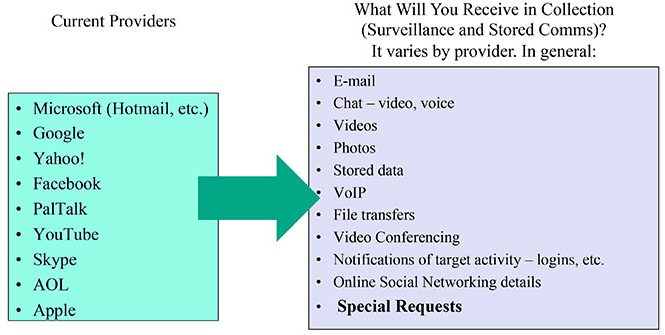
\includegraphics[width=0.7\textwidth]{images-nsa-providers.png}
    \end{center}
    % NOTE: souligner ici les différentes réactions
\end{frame}


\begin{frame}\frametitle{NSA : comment interceptent-ils les données ?}
    \textbf{Ecoutes aux points de sortie des câbles sous-marins :}
    \vspace{1em}
    \begin{center}
        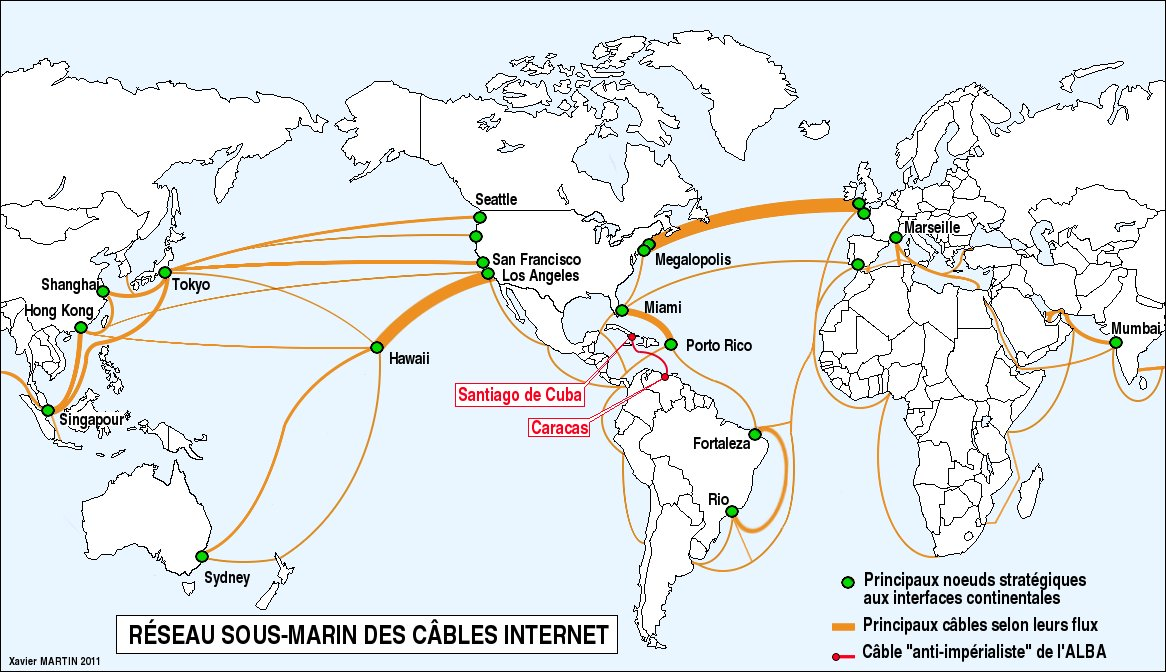
\includegraphics[width=0.8\textwidth]{images-nsa-cables.jpg}
    \end{center}
\end{frame}


\begin{frame}\frametitle{NSA : comment interceptent-ils les données ?}
    {\center \huge \bfseries Avoir des amis, c'est cool ;)}

    \vspace{1em}
    \textbf{Five Eyes} :
    \begin{itemize}
        \item Etats-unis
        \item Royaumes-unis
        \item Nouvelle-Zélande
        \item Canada
        \item Australie
    \end{itemize}
    \textbf{Nine Eyes} : + Danemark, \emph{France}, Pays-Bas et Norvége

    \textbf{Fourteen Eyes} : + Allemagne, Belgique, Italie, Espagne et Suède
\end{frame}


\begin{frame}\frametitle{WTF la France ?}
    \emph{«Je croyais que la France était pas contente de la NSA...»}
    
    Hahaha petit naïf...

    \vspace{1em}
    \begin{itemize}
        \item des interceptions administratives à la peleteuse
        \item du DPI \emph{(Deep Packet Inspection)} en \emph{masse}
        \item revente d'armes numériques (\emph{Eagle}) à des régimes totalitaires
            (Kadafi) avec quelques petites portes dérobées ;)
        \item quelques accords avec les Américains (\emph{Lustre})
        \item 70 millions de communications téléphoniques transmises à la NSA
    \end{itemize}
\end{frame}

